% ============================================================
% main.tex — QWMO Full Research Article
% Elsevier / Swarm and Evolutionary Computation Compatible
% ============================================================

\documentclass[final,5p,times,twocolumn]{elsarticle}

% ============================================================
% PACKAGES
% ============================================================

\usepackage[T1]{fontenc}
\usepackage[utf8]{inputenc}

\usepackage{amsmath}
\usepackage{amssymb}
\usepackage{amsfonts}
\usepackage{amsthm}

\usepackage{graphicx}
\usepackage{booktabs}
\usepackage{multirow}
\usepackage{array}
\usepackage{algorithm}
\usepackage{algpseudocode}
\usepackage{xcolor}
\usepackage{url}

\usepackage{tikz}
\usetikzlibrary{
    arrows.meta,
    positioning,
    backgrounds,
    calc,
    decorations.pathmorphing,
    decorations.markings
}

% ============================================================
% JOURNAL
% ============================================================

\journal{Swarm and Evolutionary Computation}

% ============================================================
% THEOREM ENVIRONMENTS
% ============================================================

\newtheorem{lemma}{Lemma}
\newtheorem{theorem}{Theorem}
\newtheorem{remark}{Remark}

% ============================================================
% DOCUMENT
% ============================================================

\begin{document}

\begin{frontmatter}

\title{
QWMO: A Quantum Wave-function Inspired Metaheuristic
for Multimodal Optimization
}

\author[inst1]{Ömer Samuk\corref{cor1}}
\cortext[cor1]{Corresponding author}
\ead{offical.samuk@gmail.com}
\ead[url]{https://orcid.org/0009-0000-5221-034X}
\ead[url]{https://github.com/OmerSamuk/QWMO}

\affiliation[inst1]{
organization={Tıp Fakültesi, Selçuk Üniversitesi},
city={Konya},
country={Türkiye}
}

% ============================================================
% ABSTRACT
% ============================================================

\begin{abstract}

This paper introduces QWMO
(Quantum Wave-function Metaheuristic Optimizer),
a quantum-inspired population-based optimization framework
designed to investigate the role of probabilistic operators
in balancing exploration and exploitation in multimodal
optimization landscapes.

The proposed framework combines three operators:
(i) Adaptive Orbital Sampling, which controls Gaussian
search dispersion according to relative solution quality;
(ii) Pauli-Inspired Exclusion, which preserves population
diversity through orthogonal displacement dynamics; and
(iii) Adaptive Quantum Escape, which enables stagnating
agents to probabilistically leave local optima through
stochastic relocation.

Unlike classical physics-inspired optimizers relying on
deterministic force interactions, QWMO models search
dynamics through wave-function-guided stochastic transitions.
Experiments on five representative CEC-style benchmark
functions in 30 dimensions with 30 independent runs indicate
that QWMO consistently outperforms its direct physics-inspired
counterparts ASO and AOS under Wilcoxon signed-rank analysis
($p<0.05$), while maintaining competitive behavior against
classical swarm-based optimizers on multimodal and hybrid
landscapes.

An ablation study further shows that QWMO's behavior emerges
from the interaction between adaptive orbital sampling,
diversity-preserving exclusion, and stochastic escape dynamics,
rather than from any single operator alone.

\end{abstract}

\begin{keyword}
metaheuristic optimization \sep
quantum-inspired optimization \sep
multimodal optimization \sep
swarm intelligence \sep
stochastic optimization \sep
Markov process
\end{keyword}

\end{frontmatter}

% ============================================================
% 1. INTRODUCTION
% ============================================================

\section{Introduction}

Metaheuristic algorithms have become one of the dominant
paradigms for black-box global optimization.
Population-based frameworks such as Particle Swarm
Optimization (PSO) \cite{kennedy1995pso}, Genetic Algorithms
(GA) \cite{goldberg1989ga}, Grey Wolf Optimizer (GWO)
\cite{mirjalili2014gwo}, and Whale Optimization Algorithm
(WOA) \cite{mirjalili2016woa} have been widely applied to
continuous, discrete, and hybrid optimization problems.

Despite their empirical success, many metaheuristic optimizers
still suffer from premature convergence, loss of diversity,
and unstable exploration--exploitation balance, particularly
in highly multimodal landscapes. This limitation becomes more
pronounced in high-dimensional search spaces, where population
collapse around local minima can substantially reduce global
search capability.

Physics-inspired optimization methods attempt to address these
issues through analogies derived from gravitational, atomic,
or thermodynamic systems. Examples include the Gravitational
Search Algorithm (GSA) \cite{rashedi2009gsa}, Atom Search
Optimization (ASO) \cite{zhao2019aso}, and Atomic Orbital
Search (AOS) \cite{azizi2021aos}. Although such methods
introduce alternative interaction mechanisms, many remain
based on deterministic force laws or globally shared search
parameters.

Recent quantum-inspired approaches have explored probabilistic
search dynamics, including Quantum-Inspired Evolutionary
Algorithms (QIEA) \cite{nowotniak2010qiea} and recent
quantum-driven metaheuristic studies such as the Quantum
Snowflake Algorithm (QSA) \cite{qsa2025}. However, many
existing quantum-inspired optimizers emphasize probabilistic
representation without explicitly integrating diversity
preservation and adaptive escape behavior within a single
operator-level framework.

Unlike studies aiming to introduce universally dominant
optimizers, the objective of QWMO is to investigate how
quantum-inspired probabilistic operators influence the
exploration--exploitation balance in multimodal optimization
landscapes.

The main contributions of this paper are summarized as follows:

\begin{itemize}
    \item A wave-function-inspired adaptive orbital sampling
    mechanism is proposed to control Gaussian search dispersion
    according to relative solution quality.

    \item A Pauli-Inspired Exclusion operator is introduced to
    preserve population diversity through orthogonal displacement
    rather than collinear repulsion.

    \item An Adaptive Quantum Escape operator is formulated to
    recover stagnating agents through probabilistic stochastic
    relocation.

    \item A probabilistic convergence perspective is developed
    using an extended-state Markov process interpretation.

    \item Comparative benchmark experiments and ablation analysis
    are conducted on representative CEC-style multimodal
    optimization functions.
\end{itemize}

The rest of the paper is organized as follows.
Section~\ref{sec:background} reviews related metaheuristic,
physics-inspired, and quantum-inspired optimization methods.
Section~\ref{sec:method} presents the proposed QWMO framework.
Section~\ref{sec:theory} discusses the probabilistic convergence
perspective. Section~\ref{sec:experiments} describes the
experimental protocol. Section~\ref{sec:results} reports the
benchmark results. Section~\ref{sec:ablation} presents the
ablation study. Section~\ref{sec:conclusion} concludes the paper.

% ============================================================
% 2. BACKGROUND
% ============================================================

\section{Background and Related Work}
\label{sec:background}

\subsection{Classical population-based metaheuristics}

Population-based metaheuristics maintain multiple candidate
solutions and update them through stochastic or rule-based
interactions. PSO models social learning through velocity-based
updates \cite{kennedy1995pso}, while GA relies on selection,
crossover, and mutation to recombine candidate solutions
\cite{goldberg1989ga}. GWO and WOA introduce biologically
inspired encircling and hunting mechanisms
\cite{mirjalili2014gwo,mirjalili2016woa}.

These algorithms are effective on many benchmark problems, but
their performance depends strongly on the structure of the
objective landscape. In particular, multimodal functions can
cause premature convergence when the population loses diversity
or when update rules repeatedly pull agents toward suboptimal
basins.

\subsection{Physics-inspired optimization}

Physics-inspired optimizers translate physical interaction
models into search operators. GSA uses gravitational attraction
between candidate solutions \cite{rashedi2009gsa}. ASO models
agent interactions through atom-like forces and Lennard-Jones
inspired pairwise dynamics \cite{zhao2019aso}. AOS uses an
atomic orbital analogy to guide agent placement through
probability density functions \cite{azizi2021aos}.

Although these approaches enrich the search process with
physical metaphors, they also introduce limitations. Pairwise
force models can be computationally expensive, and collinear
interaction dynamics may lead to oscillatory or redundant
movement. In addition, globally decaying search radii may reduce
the ability to differentiate between agents that should explore
and agents that should exploit.

\subsection{Quantum-inspired optimization}

Quantum-inspired metaheuristics use concepts such as
superposition, probabilistic representation, and tunneling as
algorithmic analogies rather than as direct physical simulation.
QIEA is a representative example, encoding solutions through
quantum-inspired probabilistic structures \cite{nowotniak2010qiea}.
Recent work such as QSA further explores quantum-driven
operators in continuous and discrete optimization settings
\cite{qsa2025}.

QWMO follows this broad quantum-inspired direction, but differs
by explicitly decomposing the search process into three
separable operators: sampling, exclusion, and escape. This
decomposition enables ablation analysis and clearer assessment
of the contribution of each mechanism.

\subsection{Diversity preservation}

Diversity preservation is a central issue in evolutionary and
swarm optimization. Exclusion mechanisms, multiswarms, niching,
and fitness sharing have been used to prevent premature
population collapse \cite{blackwell2006multiswarm,
sareni1998fitness}. Repulsive PSO variants also use attraction
and repulsion to regulate population spread
\cite{mullen2007orienteering}.

Most repulsive or exclusion-based mechanisms operate along
the collision vector between two agents. QWMO instead applies
orthogonal displacement, moving the weaker agent into a
direction perpendicular to the collision vector. This design
reduces repeated back-and-forth displacement along the same
axis and encourages spatial diversification.

% ============================================================
% 3. METHOD
% ============================================================

\section{Quantum Wave-function Metaheuristic Optimizer}
\label{sec:method}

Let the search domain be a bounded hyper-rectangle
$\Omega=[\ell,u]^D$, where $D$ is the dimensionality.
The population at iteration $t$ is denoted by
$X(t)=\{\mathbf{x}_1(t),\dots,\mathbf{x}_N(t)\}$.
Each agent $\mathbf{x}_i(t)\in\Omega$ has an associated
objective value $f(\mathbf{x}_i)$.
The best-so-far solution is denoted by $\mathbf{x}^{*}$.

QWMO applies three operators at each iteration:
Adaptive Orbital Sampling, Pauli-Inspired Exclusion, and
Adaptive Quantum Escape. The terminology is used as an
optimization analogy rather than a direct physical simulation
of quantum systems.

\subsection{Adaptive Orbital Sampling}

Each agent samples a candidate position from a Gaussian
distribution centered at its current location:
\begin{equation}
\mathbf{x}'_i \sim
\mathcal{N}\left(\mathbf{x}_i,\sigma_i^2(t)\mathbf{I}\right).
\end{equation}

The relative quality of agent $i$ is defined as
\begin{equation}
q_i =
\frac{f_{\mathrm{worst}}-f(\mathbf{x}_i)}
{f_{\mathrm{worst}}-f_{\mathrm{best}}+\epsilon},
\end{equation}
where $q_i\in[0,1]$, $f_{\mathrm{best}}$ is the best value in
the current population, $f_{\mathrm{worst}}$ is the worst value,
and $\epsilon$ is a small numerical stabilizer.

The maximum orbital radius and decay coefficient are given by
\begin{equation}
\sigma_{\max,i}=\gamma(u-\ell)(2-q_i),
\qquad
c_i=c_{\mathrm{base}}q_i.
\end{equation}

The sampling radius is then computed as
\begin{equation}
\sigma_i(t)=
\max\left\{
\sigma_{\max,i}
\exp\left(-c_i\frac{t}{T_{\max}}\right),
\sigma_{\lfloor}
\right\},
\end{equation}
where $\sigma_{\lfloor}=10^{-8}$ ensures a strictly positive
sampling variance.

High-quality agents contract more rapidly and perform local
refinement, whereas low-quality agents retain wider orbits and
continue exploring broader regions of the search space.

\subsection{Pauli-Inspired Exclusion}

If two agents violate the exclusion radius,
\begin{equation}
\|\mathbf{x}_i-\mathbf{x}_j\|<\varepsilon,
\end{equation}
the weaker agent is displaced orthogonally relative to the
collision vector.

Let $\mathbf{x}_b$ denote the weaker agent and $\mathbf{x}_g$
the better agent. Define
\begin{equation}
\mathbf{v}=\mathbf{x}_b-\mathbf{x}_g.
\end{equation}
A random vector $\mathbf{r}\sim\mathcal{N}(0,\mathbf{I})$ is
projected onto the subspace orthogonal to $\mathbf{v}$:
\begin{equation}
\mathbf{p}
=
\mathbf{r}
-
\frac{\mathbf{r}^{\top}\mathbf{v}}
{\|\mathbf{v}\|^2+10^{-10}}
\mathbf{v}.
\end{equation}

The weaker agent is updated as
\begin{equation}
\mathbf{x}_b
\leftarrow
\mathrm{clip}
\left(
\mathbf{x}_b+
\alpha\frac{\mathbf{p}}{\|\mathbf{p}\|+10^{-10}},
\ell,u
\right),
\end{equation}
where
\begin{equation}
\alpha\sim\mathcal{U}(0.5\varepsilon,1.5\varepsilon).
\end{equation}

Collision detection is implemented using a k-d tree
\cite{bentley1975multidimensional}, reducing neighborhood
search complexity from a naive $\mathcal{O}(N^2)$ pairwise
scan to approximately $\mathcal{O}(N\log N)$ in low and
moderate dimensions.

\subsection{Adaptive Quantum Escape}

Each agent maintains a stagnation counter $k_i$.
When $k_i>k_s$, the agent becomes eligible for probabilistic
escape:
\begin{equation}
P_{\mathrm{esc}}(t)
=
\exp\left(-2\kappa(t)L_{\mathrm{norm}}\right),
\end{equation}
where
\begin{equation}
\kappa(t)=\kappa_0\frac{t}{T_{\max}},
\qquad
L_{\mathrm{norm}}
=
\frac{\|\mathbf{x}_i-\mathbf{x}^{*}\|}{L_{\max}}.
\end{equation}

The destination is generated through a hybrid stochastic rule:
\begin{equation}
\mathbf{x}'_i
=
\beta(\mathbf{x}^{*}+\boldsymbol{\eta})
+
(1-\beta)\mathbf{x}_r,
\end{equation}
where
\[
\beta\sim\mathcal{U}[0,1],
\qquad
\boldsymbol{\eta}\sim\mathcal{N}(0,\sigma_{\mathrm{noise}}^2\mathbf{I}),
\qquad
\mathbf{x}_r\sim\mathcal{U}[\ell,u]^D.
\]

The global-best component provides directional guidance, while
the random component preserves long-range exploration.

% ============================================================
% qwmo_figure_final.tex
% Figure 1 — QWMO Operators
% Elsevier-compatible TikZ figure
% ============================================================

\begin{figure*}[t]
\centering

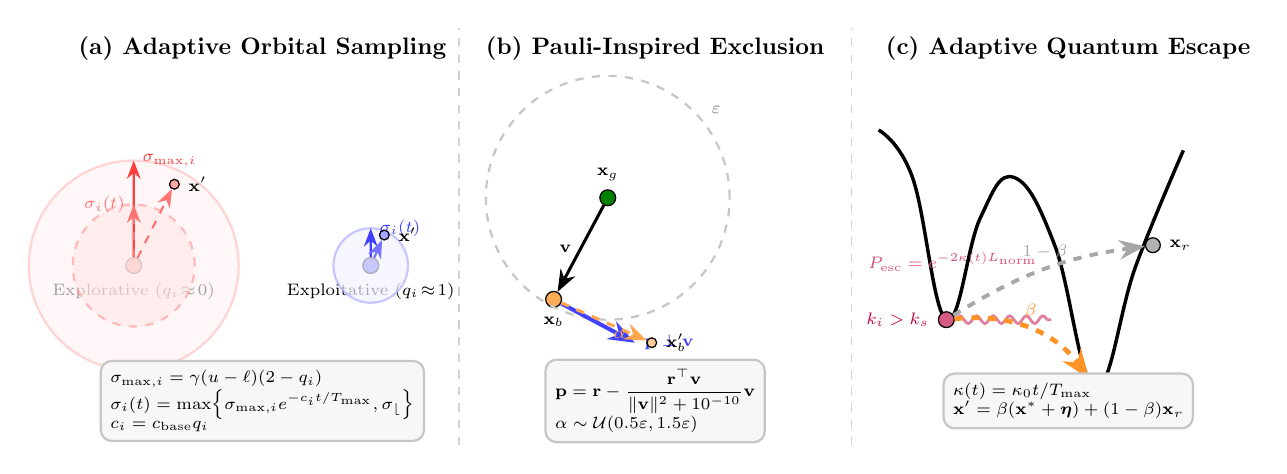
\begin{tikzpicture}[
    >=Stealth,
    thick,
    scale=0.86,
    every node/.style={scale=0.86},
    agent/.style={
        circle,
        draw=black,
        line width=0.45pt,
        inner sep=2.35pt
    },
    boxnote/.style={
        draw=gray!45,
        fill=gray!6,
        rounded corners,
        font=\scriptsize,
        align=left,
        inner sep=4pt
    }
]

% ============================================================
% PANEL SEPARATORS
% ============================================================

\draw[gray!35, dashed, line width=0.6pt]
    (5.8,-1.15) -- (5.8,5.0);

\draw[gray!35, dashed, line width=0.6pt]
    (11.6,-1.15) -- (11.6,5.0);

% ============================================================
% PANEL A — ADAPTIVE ORBITAL SAMPLING
% ============================================================

\node[font=\bfseries]
    at (2.9,4.7)
    {(a) Adaptive Orbital Sampling};

% Explorative agent
\node[
    agent,
    fill=red!55,
    label={[font=\scriptsize]below:
    Explorative ($q_i\!\approx\!0$)}
]
    (explore) at (1.0,1.5) {};

% Wide orbital
\draw[red!25, fill=red!5, opacity=0.65]
    (explore) circle (1.55);

\draw[red!45, dashed, fill=red!10, opacity=0.55]
    (explore) circle (0.9);

\draw[->, red!75]
    (explore) -- ++(0,1.55)
    node[right, font=\scriptsize]
    {$\sigma_{\max,i}$};

\draw[->, red!55, dashed]
    (explore) -- ++(0,0.9)
    node[left, font=\scriptsize]
    {$\sigma_i(t)$};

% Sample point from broad orbital
\node[
    agent,
    fill=red!35,
    inner sep=1.45pt,
    label={[font=\scriptsize]right:$\mathbf{x}'$}
]
    (sampleA) at (1.6,2.7) {};

\draw[->, red!55, dashed]
    (explore) -- (sampleA);

% Exploitative agent
\node[
    agent,
    fill=blue!60,
    label={[font=\scriptsize]below:
    Exploitative ($q_i\!\approx\!1$)}
]
    (exploit) at (4.5,1.5) {};

% Narrow orbital
\draw[blue!30, fill=blue!5, opacity=0.7]
    (exploit) circle (0.55);

\draw[->, blue!75]
    (exploit) -- ++(0,0.55)
    node[right, font=\scriptsize]
    {$\sigma_i(t)$};

% Sample point from narrow orbital
\node[
    agent,
    fill=blue!35,
    inner sep=1.45pt,
    label={[font=\scriptsize]right:$\mathbf{x}'$}
]
    (sampleB) at (4.7,1.95) {};

\draw[->, blue!55, dashed]
    (exploit) -- (sampleB);

% Formula box
\node[boxnote]
    at (2.9,-0.5)
{
$\sigma_{\max,i}=\gamma(u-\ell)(2-q_i)$\\
$\sigma_i(t)=
\max\!\left\{\sigma_{\max,i}e^{-c_i t/T_{\max}},
\sigma_{\lfloor}\right\}$\\
$c_i=c_{\mathrm{base}}q_i$
};

% ============================================================
% PANEL B — PAULI-INSPIRED EXCLUSION
% ============================================================

\node[font=\bfseries]
    at (8.7,4.7)
    {(b) Pauli-Inspired Exclusion};

% Better agent
\node[
    agent,
    fill=green!50!black,
    label={[font=\scriptsize]above:$\mathbf{x}_g$}
]
    (xg) at (8.0,2.5) {};

% Weaker agent
\node[
    agent,
    fill=orange!65,
    label={[font=\scriptsize]below:$\mathbf{x}_b$}
]
    (xb) at (7.2,1.0) {};

% Exclusion radius
\draw[gray!45, dashed]
    (xg) circle (1.8);

\node[font=\scriptsize, color=gray]
    at (9.6,3.8)
    {$\varepsilon$};

% Collision vector
\draw[->, black, line width=1.1pt]
    (xg) -- (xb)
    node[midway, left, font=\scriptsize]
    {$\mathbf{v}$};

% Orthogonal displacement
\draw[->, blue!75, line width=1.45pt]
    (xb) -- ++(1.2,-0.64)
    node[right, font=\scriptsize]
    {$\mathbf{p}\perp\mathbf{v}$};

% New position
\node[
    agent,
    fill=orange!40,
    inner sep=1.45pt,
    label={[font=\scriptsize]right:$\mathbf{x}_b'$}
]
    (xbnew) at (8.65,0.36) {};

\draw[
    ->,
    orange!70,
    dashed,
    line width=1.1pt
]
    (xb) -- (xbnew)
    node[midway, below right, font=\scriptsize]
    {$\alpha$};

% Formula box
\node[boxnote]
    at (8.7,-0.5)
{
$\mathbf{p}=
\mathbf{r}-
\dfrac{\mathbf{r}^{\top}\mathbf{v}}
{\|\mathbf{v}\|^2+10^{-10}}\mathbf{v}$\\
$\alpha\sim\mathcal{U}(0.5\varepsilon,1.5\varepsilon)$
};

% ============================================================
% PANEL C — ADAPTIVE QUANTUM ESCAPE
% ============================================================

\node[font=\bfseries]
    at (14.8,4.7)
    {(c) Adaptive Quantum Escape};

% Energy landscape
\draw[black, line width=1.25pt]
plot[smooth, tension=0.7] coordinates {
    (12.0,3.5)
    (12.5,2.8)
    (13.0,0.7)
    (13.5,2.2)
    (14.0,2.8)
    (14.6,1.8)
    (15.2,-0.3)
    (15.8,1.5)
    (16.5,3.2)
};

% Stagnating agent
\node[
    agent,
    fill=purple!65,
    label={[font=\scriptsize, color=purple]left:$k_i>k_s$}
]
    (trapped) at (13.0,0.7) {};

% Escape probability
\node[
    font=\scriptsize,
    color=purple!70
]
    at (13.1,1.55)
{
$P_{\mathrm{esc}}=e^{-2\kappa(t)L_{\mathrm{norm}}}$
};

% Global best
\node[
    agent,
    fill=black,
    inner sep=3pt,
    label={[font=\scriptsize]below:$\mathbf{x}^{*}$}
]
    (gopt) at (15.2,-0.3) {};

% Random exploration target
\node[
    agent,
    fill=gray!60,
    inner sep=2.2pt,
    label={[font=\scriptsize]right:$\mathbf{x}_r$}
]
    (randp) at (16.05,1.8) {};

% Wavy escape path
\draw[
    purple!50,
    line width=1pt,
    decoration={
        snake,
        amplitude=1.4pt,
        segment length=6pt
    },
    decorate
]
    (trapped) -- (14.55,0.7);

% Hybrid stochastic relocation arrows
\draw[
    ->,
    orange!85,
    line width=1.7pt,
    dashed,
    bend left=30
]
    (trapped) to
    node[above, font=\scriptsize, color=orange!80]
    {$\beta$}
    (gopt);

\draw[
    ->,
    gray!70,
    line width=1.4pt,
    dashed,
    bend left=12
]
    (trapped) to
    node[above, font=\scriptsize]
    {$1-\beta$}
    (randp);

% Formula box
\node[boxnote]
    at (14.8,-0.5)
{
$\kappa(t)=\kappa_0 t/T_{\max}$\\
$\mathbf{x}'=\beta(\mathbf{x}^{*}+\boldsymbol{\eta})
+(1-\beta)\mathbf{x}_r$
};

\end{tikzpicture}

\caption{
Schematic illustration of the three operators composing QWMO.
(a) Adaptive Orbital Sampling dynamically adjusts the Gaussian
sampling radius according to solution quality, balancing
exploration and exploitation.
(b) Pauli-Inspired Exclusion applies orthogonal displacement
when neighboring agents violate the exclusion radius
$\varepsilon$, promoting spatial diversity.
(c) Adaptive Quantum Escape enables stagnating agents
to leave local minima through probabilistic
$\beta$-hybrid stochastic relocation between
the global-best region and random exploration targets.
The terminology is used as an optimization analogy rather than
a direct physical simulation of quantum systems.
The combined interaction of the three operators establishes
the exploration--exploitation balance of QWMO.
}
\label{fig:qwmo_operators}

\end{figure*}

\subsection{Algorithmic procedure}

\begin{algorithm}[t]
\caption{QWMO}
\label{alg:qwmo}
\begin{algorithmic}[1]
\Require $N,T_{\max},\varepsilon_r,k_s,\gamma,c_{\mathrm{base}},\kappa_0,\eta_r$
\Ensure Best-so-far solution $\mathbf{x}^{*}$
\State Initialize $X$ uniformly in $[\ell,u]^D$
\State Evaluate $f(\mathbf{x}_i)$ for all agents
\State $\mathbf{x}^{*}\gets \arg\min_i f(\mathbf{x}_i)$
\State $k_i\gets 0$ for all agents
\State $\varepsilon\gets \varepsilon_r(u-\ell)$
\State $\sigma_{\mathrm{noise}}\gets \eta_r(u-\ell)$
\State $L_{\max}\gets \sqrt{D}(u-\ell)$
\For{$t=1$ to $T_{\max}$}
    \State Compute $f_{\mathrm{best}}$ and $f_{\mathrm{worst}}$
    \For{each agent $i$}
        \State Compute $q_i$, $\sigma_{\max,i}$, $c_i$, and $\sigma_i(t)$
        \State Sample $\mathbf{x}'_i\sim\mathcal{N}(\mathbf{x}_i,\sigma_i^2(t)\mathbf{I})$
        \State Clip $\mathbf{x}'_i$ to $[\ell,u]^D$
        \If{$f(\mathbf{x}'_i)<f(\mathbf{x}_i)$}
            \State $\mathbf{x}_i\gets \mathbf{x}'_i$
            \State $k_i\gets 0$
        \Else
            \State $k_i\gets k_i+1$
        \EndIf
    \EndFor
    \State Build k-d tree and query pairs within $\varepsilon$
    \For{each colliding pair}
        \State Apply Pauli-Inspired Exclusion to the weaker agent
    \EndFor
    \For{each agent with $k_i>k_s$}
        \State Compute $P_{\mathrm{esc}}(t)$
        \If{$\mathcal{U}(0,1)<P_{\mathrm{esc}}(t)$}
            \State Apply Adaptive Quantum Escape
            \State $k_i\gets 0$
        \EndIf
    \EndFor
    \State Update $\mathbf{x}^{*}$ if a better solution is found
\EndFor
\State \Return $\mathbf{x}^{*}$
\end{algorithmic}
\end{algorithm}

% ============================================================
% 4. THEORY
% ============================================================

\section{Theoretical Analysis}
\label{sec:theory}

The probabilistic dynamics of QWMO can be interpreted within
an extended-state Markov process. Let
$\mathcal{S}\subset\mathbb{R}^D$ denote the bounded search
space and let $P(\mathbf{x},A)$ denote the stochastic
transition kernel induced by the QWMO update operators for
a measurable set $A\subseteq\mathcal{S}$.

Since the Adaptive Quantum Escape operator depends on the
stagnation counter, the state is augmented as
\begin{equation}
s_i(t)=(\mathbf{x}_i(t),k_i(t)).
\end{equation}
This extended representation preserves the Markov property
because future transitions depend on the current position and
current stagnation counter, not on the full historical trajectory.

\begin{lemma}[Positive reachability]
If $\sigma_i(t)\geq \sigma_{\lfloor}>0$, then the Adaptive
Orbital Sampling operator assigns non-zero probability to
every measurable neighborhood within the bounded search domain.
\end{lemma}

\begin{proof}
The truncated Gaussian sampling kernel has strictly positive
density over the bounded search domain when its variance is
bounded below by $\sigma_{\lfloor}>0$. Therefore, for any
measurable set $A$ with positive Lebesgue measure,
$P(\mathbf{x},A)>0$.
\end{proof}

\begin{lemma}[Stagnation escape]
The Adaptive Quantum Escape operator prevents permanent
absorbing stagnation states under the idealized stochastic
model.
\end{lemma}

\begin{proof}
Whenever an agent fails to improve, its stagnation counter
increases. Once the counter exceeds $k_s$, the escape operator
is activated with strictly positive probability as long as
$\kappa(t)$ and $L_{\mathrm{norm}}$ are finite. Hence, stagnant
states retain non-zero probability of leaving their local region.
\end{proof}

\begin{theorem}[Practical stochastic convergence behavior]
Under bounded-domain assumptions and strictly positive
transition probabilities induced by the sampling and escape
operators, QWMO exhibits practical stochastic convergence
behavior toward high-quality regions of the search space.
\end{theorem}

\begin{remark}
This result is stated as a probabilistic convergence perspective
rather than a full asymptotic global convergence proof. A complete
Harris recurrence argument would require explicit drift and
minorization conditions, which are left for future theoretical work.
\end{remark}

% ============================================================
% 5. EXPERIMENTAL SETUP
% ============================================================

\section{Experimental Setup}
\label{sec:experiments}

\subsection{Benchmark functions}

The proposed algorithm was evaluated on five representative
CEC-style benchmark functions:
Sphere (F1), Schwefel (F5), Rastrigin (F10), Hybrid Function
(F20), and Composition Function (F28). These functions cover
unimodal, multimodal, hybrid, and composition landscapes.

All experiments were conducted in 30 dimensions using
30 independent runs with distinct random seeds. The maximum
iteration budget was fixed at
\[
T_{\max}=300000.
\]

\subsection{Compared algorithms}

QWMO was compared against six baseline algorithms:
PSO, GA, GWO, WOA, ASO, and AOS. These baselines were selected
to represent classical swarm intelligence, evolutionary search,
and physics-inspired optimization.

\subsection{Parameter settings}

The QWMO parameters were fixed as follows:
\[
\gamma=0.05,\quad
c_{\mathrm{base}}=5,\quad
\kappa_0=8,\quad
\varepsilon_r=0.05,\quad
k_s=10,\quad
\eta_r=0.001.
\]

The population size was fixed at $N=50$ for all algorithms.

\subsection{Statistical analysis}

Performance is reported as mean fitness $\pm$ standard deviation
over 30 independent runs. Pairwise statistical significance
between QWMO and each competing algorithm was evaluated using
Wilcoxon signed-rank analysis with significance threshold
$p<0.05$.

Pairwise Wilcoxon signed-rank analysis was adopted as the
primary statistical comparison framework in this preliminary
study. No global rank-based post-hoc procedure is reported.

% ============================================================
% 6. RESULTS
% ============================================================

\section{Results and Discussion}
\label{sec:results}

Table~\ref{tab:main_results} reports the mean and standard
deviation of the best fitness values obtained over 30 runs.
Lower values indicate better performance.

\begin{table*}[t]
\centering
\caption{
Mean $\pm$ standard deviation of best fitness values over
30 independent runs in 30 dimensions.
Bold values indicate the best result in each column.
}
\label{tab:main_results}
\renewcommand{\arraystretch}{1.12}
\resizebox{\textwidth}{!}{
\begin{tabular}{lccccc}
\toprule
\textbf{Algorithm}
& \textbf{F1 Sphere}
& \textbf{F5 Schwefel}
& \textbf{F10 Rastrigin}
& \textbf{F20 Hybrid}
& \textbf{F28 Composition} \\
\midrule
PSO
& \textbf{0.000e+00 $\pm$ 0.00e+00}
& 4.619e+03 $\pm$ 7.83e+02
& 5.888e+01 $\pm$ 2.05e+01
& 1.647e+02 $\pm$ 8.06e+00
& 1.066e+04 $\pm$ 1.13e+02 \\
GA
& 2.717e-05 $\pm$ 1.17e-05
& \textbf{3.158e+02 $\pm$ 2.25e+02}
& 8.339e-06 $\pm$ 3.41e-06
& \textbf{1.486e+02 $\pm$ 1.42e-09}
& \textbf{1.055e+04 $\pm$ 2.78e-07} \\
GWO
& \textbf{0.000e+00 $\pm$ 0.00e+00}
& 9.255e+03 $\pm$ 2.62e+02
& \textbf{0.000e+00 $\pm$ 0.00e+00}
& 1.486e+02 $\pm$ 1.14e-02
& 1.112e+04 $\pm$ 5.26e+01 \\
WOA
& \textbf{0.000e+00 $\pm$ 0.00e+00}
& 4.038e+03 $\pm$ 9.52e+02
& 1.587e+02 $\pm$ 4.51e+01
& 1.817e+02 $\pm$ 2.02e+01
& 1.055e+04 $\pm$ 5.97e-10 \\
ASO
& 6.668e+02 $\pm$ 2.49e+03
& 3.871e+03 $\pm$ 6.83e+02
& 1.308e+02 $\pm$ 2.69e+01
& 1.805e+02 $\pm$ 1.12e+01
& 1.059e+04 $\pm$ 6.83e+01 \\
AOS
& 3.622e+03 $\pm$ 5.39e+02
& 7.258e+03 $\pm$ 2.75e+02
& 1.877e+02 $\pm$ 1.48e+01
& 2.074e+02 $\pm$ 6.96e+00
& 1.060e+04 $\pm$ 8.96e+00 \\
\textbf{QWMO}
& 1.082e+00 $\pm$ 2.65e-01
& 3.028e+03 $\pm$ 4.23e+02
& 9.023e+00 $\pm$ 2.13e+00
& 1.506e+02 $\pm$ 6.95e-01
& 1.059e+04 $\pm$ 2.67e+01 \\
\bottomrule
\end{tabular}
}
\end{table*}

QWMO consistently improves over the physics-inspired baselines
ASO and AOS on most benchmark functions. In particular, the
large performance gap on F10 Rastrigin indicates that the
adaptive escape mechanism improves search behavior on highly
multimodal landscapes.

At the same time, QWMO does not dominate all classical
baselines. GA obtains the strongest results on several
functions, and PSO/GWO achieve exact or near-exact convergence
on the unimodal Sphere function. These results support a
mechanism-focused interpretation: QWMO is not a universal
replacement for classical optimizers, but a probabilistic
framework designed to enhance exploration and escape behavior
in multimodal settings.

Table~\ref{tab:wilcoxon} reports pairwise Wilcoxon comparisons
between QWMO and each competitor.

\begin{table*}[t]
\centering
\caption{
Wilcoxon signed-rank test results with QWMO as reference.
Symbol $+$ indicates QWMO is significantly better;
$-$ indicates the competitor is significantly better;
$\approx$ indicates no statistically significant difference
at $p<0.05$.
}
\label{tab:wilcoxon}
\renewcommand{\arraystretch}{1.12}
\begin{tabular}{lccccc}
\toprule
\textbf{vs. QWMO}
& \textbf{F1}
& \textbf{F5}
& \textbf{F10}
& \textbf{F20}
& \textbf{F28} \\
\midrule
PSO & $-$ & $+$ & $+$ & $+$ & $+$ \\
GA  & $-$ & $-$ & $-$ & $-$ & $-$ \\
GWO & $-$ & $+$ & $-$ & $-$ & $+$ \\
WOA & $-$ & $+$ & $+$ & $+$ & $-$ \\
ASO & $+$ & $+$ & $+$ & $+$ & $\approx$ \\
AOS & $+$ & $+$ & $+$ & $+$ & $+$ \\
\bottomrule
\end{tabular}
\end{table*}

The Wilcoxon results show that QWMO is statistically stronger
than AOS across all five functions and stronger than ASO on
four out of five functions. This supports the claim that the
proposed operator combination improves over closely related
physics-inspired baselines. Against mature classical optimizers,
QWMO is competitive but not uniformly superior.

% ============================================================
% 7. ABLATION
% ============================================================

\section{Ablation Study}
\label{sec:ablation}

To isolate the contribution of each operator, three nested
configurations were evaluated:

\begin{itemize}
    \item \textbf{Orbital Only}: Adaptive Orbital Sampling alone.
    \item \textbf{Orbital + Pauli}: Adaptive Orbital Sampling and
    Pauli-Inspired Exclusion.
    \item \textbf{Full QWMO}: all three operators enabled.
\end{itemize}

The experimental protocol mirrors the main benchmark:
30 independent runs in 30 dimensions.

\begin{table*}[t]
\centering
\caption{
Ablation study results for QWMO variants
(mean $\pm$ standard deviation, 30D, 30 runs).
Bold values indicate the best ablation configuration.
}
\label{tab:ablation}
\renewcommand{\arraystretch}{1.12}
\resizebox{\textwidth}{!}{
\begin{tabular}{lccccc}
\toprule
\textbf{Configuration}
& \textbf{F1 Sphere}
& \textbf{F5 Schwefel}
& \textbf{F10 Rastrigin}
& \textbf{F20 Hybrid}
& \textbf{F28 Composition} \\
\midrule
Orbital Only
& \textbf{5.45e-02 $\pm$ 3.62e-03}
& 3.13e+03 $\pm$ 2.08e+02
& 5.22e+01 $\pm$ 7.54e+00
& 1.61e+02 $\pm$ 2.34e+00
& \textbf{1.055e+04 $\pm$ 1.62e-03} \\
Orbital + Pauli
& 8.08e-02 $\pm$ 7.71e-03
& 3.13e+03 $\pm$ 2.08e+02
& 5.22e+01 $\pm$ 7.54e+00
& 1.61e+02 $\pm$ 2.34e+00
& 1.055e+04 $\pm$ 3.71e-03 \\
Full QWMO
& 5.61e-01 $\pm$ 1.06e-01
& \textbf{2.09e+03 $\pm$ 3.28e+02}
& \textbf{1.40e+00 $\pm$ 9.02e-01}
& \textbf{1.50e+02 $\pm$ 6.56e-02}
& 1.055e+04 $\pm$ 3.91e-02 \\
\bottomrule
\end{tabular}
}
\end{table*}

The Orbital Only configuration provides a strong local
exploitation baseline but stagnates on multimodal landscapes.
Adding Pauli-Inspired Exclusion does not produce a measurable
improvement at $D=30$. This behavior is explained by geometric
sparsity: with $\varepsilon_r=0.05$ and a function range
approximately spanning $[-100,100]^D$, the exclusion radius is
$\varepsilon=0.05\times200=10$, while the search-space diameter is
\[
L_{\max}\approx \sqrt{30}\times200\approx1095.
\]
Thus, agents distributed across a high-dimensional domain rarely
fall within the exclusion radius. This confirms that the Pauli
operator requires an adaptive radius $\varepsilon(t)$ to be more
effective in high-dimensional search spaces.

The Full QWMO configuration substantially improves performance
on multimodal and hybrid functions. On F10 Rastrigin, the mean
error decreases from $52.20$ to $1.40$, while on F5 Schwefel it
decreases from approximately $3126$ to $2088$. These results
indicate that Adaptive Quantum Escape is the primary contributor
to performance gains on deceptive landscapes.

However, the Full QWMO configuration performs worse on Sphere
and does not improve the Composition function. This trade-off
is consistent with an exploration-oriented design: stochastic
escape improves recovery from local minima, but can reduce
fine precision on smooth unimodal surfaces or fail to resolve
highly structured composition landscapes.

% ============================================================
% 8. CONCLUSION
% ============================================================

\section{Conclusion}
\label{sec:conclusion}

This paper presented QWMO, a quantum wave-function inspired
metaheuristic framework for multimodal optimization. The
algorithm combines Adaptive Orbital Sampling, Pauli-Inspired
Exclusion, and Adaptive Quantum Escape within a unified
probabilistic search process.

The experimental results show that QWMO consistently improves
over its direct physics-inspired counterparts ASO and AOS, while
remaining competitive with established swarm-based optimizers
on multimodal and hybrid functions. The ablation study indicates
that the strength of QWMO does not arise from a single operator,
but from the interaction between adaptive orbital sampling,
diversity-preserving exclusion, and stochastic escape dynamics.

Several limitations remain. The fixed exclusion radius is not
sufficiently effective in sparse high-dimensional populations,
and the current escape policy does not materially improve the
hardest composition landscape. Future work will investigate
adaptive exclusion radii, larger benchmark suites, high-dimensional
scalability, and stronger stochastic convergence guarantees based
on Harris recurrence theory.

% ============================================================
% ACKNOWLEDGMENT
% ============================================================

\section*{Acknowledgment}

The author used AI-assisted tools for language refinement,
debugging support, and manuscript editing under full human
supervision and intellectual responsibility.

% ============================================================
% REFERENCES
% ============================================================

\bibliographystyle{elsarticle-num}
\bibliography{references_final}

\end{document}